% include the figures path relative to the master file
\graphicspath{ {./content/method/figures/visual_cues/} {./content/method/figures/}}

\section{Description of the segmentation methodology} 

Optimization methodologies offer a standardized manner to approach segmentation by minimizing an application-driven cost function~\cite{cremers2007review}.
\Cref{fig:method} illustrates a generic representation of the segmentation strategy here adopted to delineate breast tissues or lesions in \ac{us} images. 
The overall segmentation can be seen as a three-steps strategy: 
(1) a mapping of the image into a discrete set of elements $\mathcal{S}$, 
(2) the optimization stage which is formulated as a \emph{metric labelling} problem, 
and (3) a re-mapping the labels obtained from the previous stage to produce the final delineation. 

\begin{figure}[htpb]
  \centering
  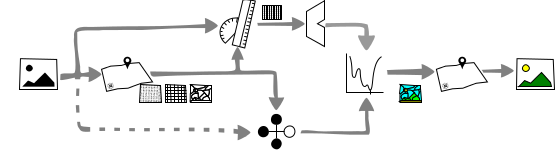
\includegraphics[width=0.9\linewidth]{method}
  \caption{Conceptual block representation of the segmentation methodology}
  \label{fig:method}
\end{figure}


In order to formulate the segmentation like a metric labelling problem, the image is conceived as a discrete set of elements $\mathcal{S}$ that need to be labelled using a label $l$ from the labelling set $\mathcal{L}$ 
(i.e.\, $\mathcal{L} = \{\text{lesion}, \overline{\text{lesion}}\}$ 
or $\mathcal{L} = \{\text{lungs}, \text{fat},\,\cdots\,, \text{lesion}\}$).
Let $\mathcal{W}$ be all the possible labelling configurations of the set $\mathcal{S}$, given $\mathcal{L}$.
Let $U(\cdot)$ be a cost function encoding the goodness of the labelling configuration $\omega \in \mathcal{W}$ based on the appearance of the elements in $\mathcal{S}$, their inner relation and some designing constraints.
Then, the desired segmentation $\hat{\omega}$ corresponds to the labelling configuration that minimizes this cost function, as described in \Cref{eq:costMin}.

\begin{equation}
\hat{\omega} = \arg \min_{\substack{\omega}} \,U(\omega)
\label{eq:costMin}
\end{equation}

It is worth to mention here that not all the minimization strategies are applicable or adequate to find $\hat{\omega}$.
The convenience of a particular minimization strategy is determined by the nature of $U(\cdot)$ and $\mathcal{W}$ (see \cref{sec:method:min}).

This goodness measure $U(\cdot)$ must be defined to take into account the appearance of the target region, its relation with other regions and other designing constraints.
\Cref{eq:labelingeq} describes this cost function as the combination of two independent costs that need to be simultaneously minimized as a whole.

\begin{equation}
  U(\omega) = \sum_{s\in s} D_s(\omega_s) + \sum_{s}\sum_{r \in \mathcal{N}_{s}} V_{s,r}(\omega_s,\omega_r)
  \label{eq:labelingeq}
\end{equation}

Where, the left hand side of the expression integrates the so-called \emph{data} term, while the right hand side integrates the \emph{pairwise} term, which is also referred as the \emph{smoothing} term.
Both terms are shaped by $\mathcal{S}$ and evaluated in the labelling space $\mathcal{W}$.
\Cref{fig:methodterms} uses the problem of delineating the tissues present in a \ac{bus} image to represent the working principles of the data and pairwise terms in \cref{eq:labelingeq}.

\begin{figure}
    \centering
    \begin{subfigure}[b]{0.19\textwidth}
        \centering
        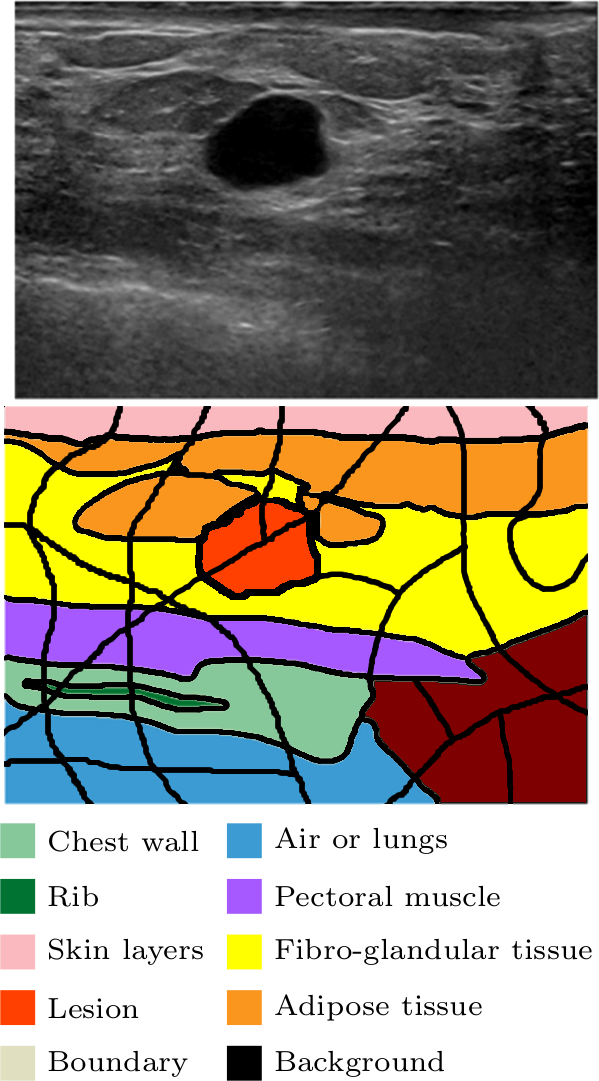
\includegraphics[width=\textwidth]{problem}
        \caption{{\small Problem definition}}    
        \label{fig:methodTerms:problem}
    \end{subfigure}
    \hfill
    \begin{subfigure}[b]{0.39\textwidth}  
        \centering 
        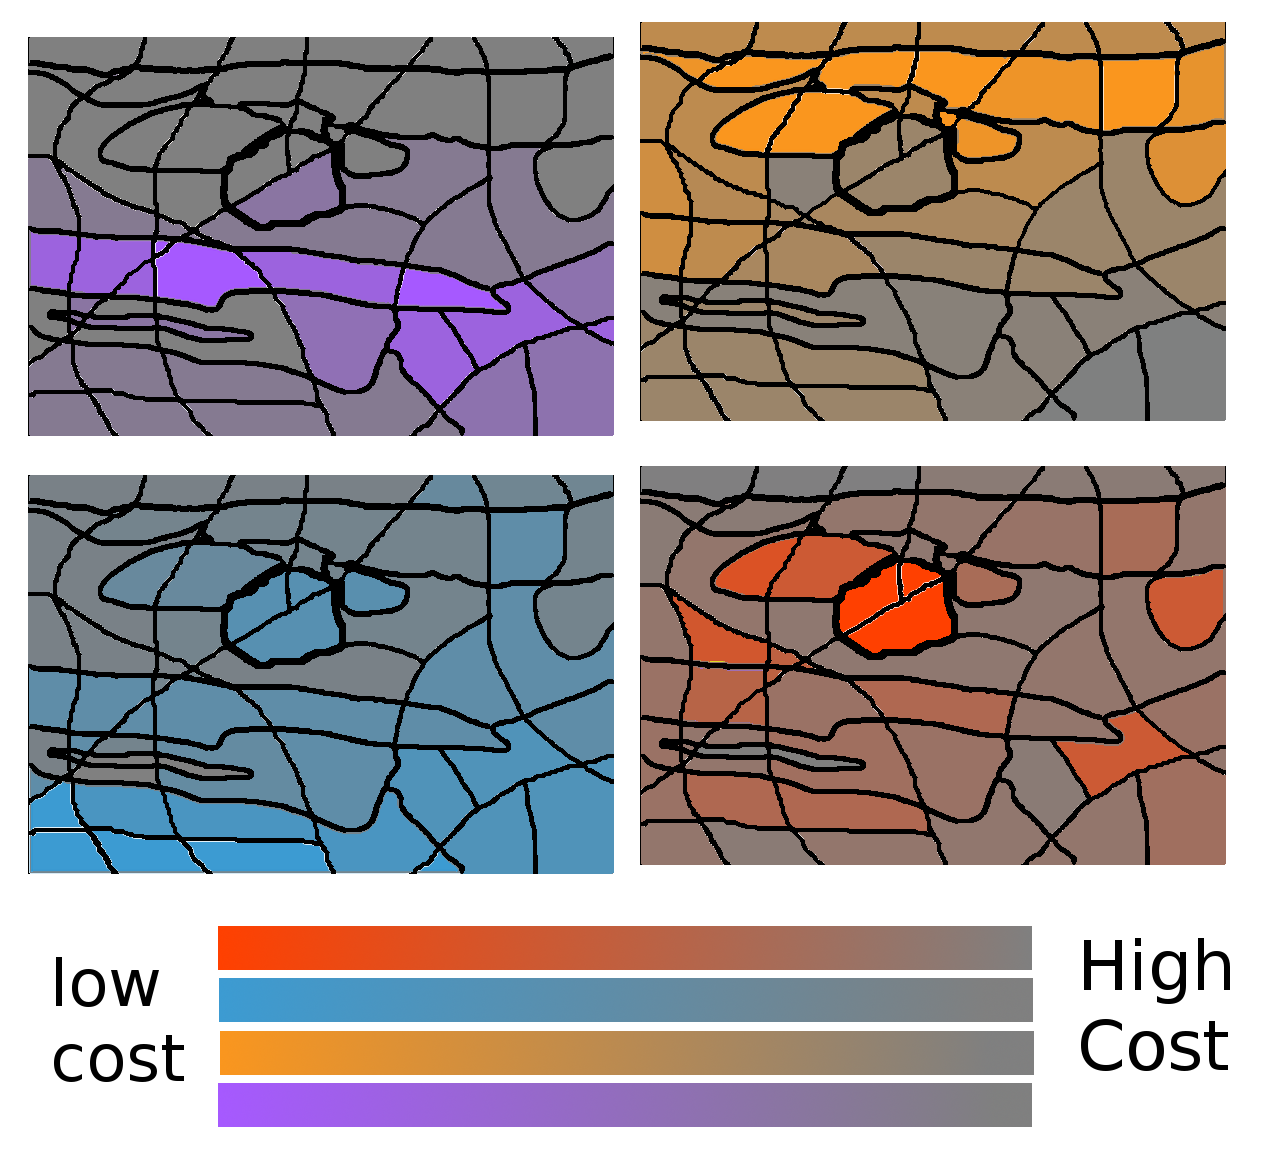
\includegraphics[width=\textwidth]{data}
        \caption[]%
        {{\small Data term}}    
        \label{fig:methodTerms:data}
    \end{subfigure}
    \hfill
    \begin{subfigure}[b]{0.39\textwidth}   
        \centering 
        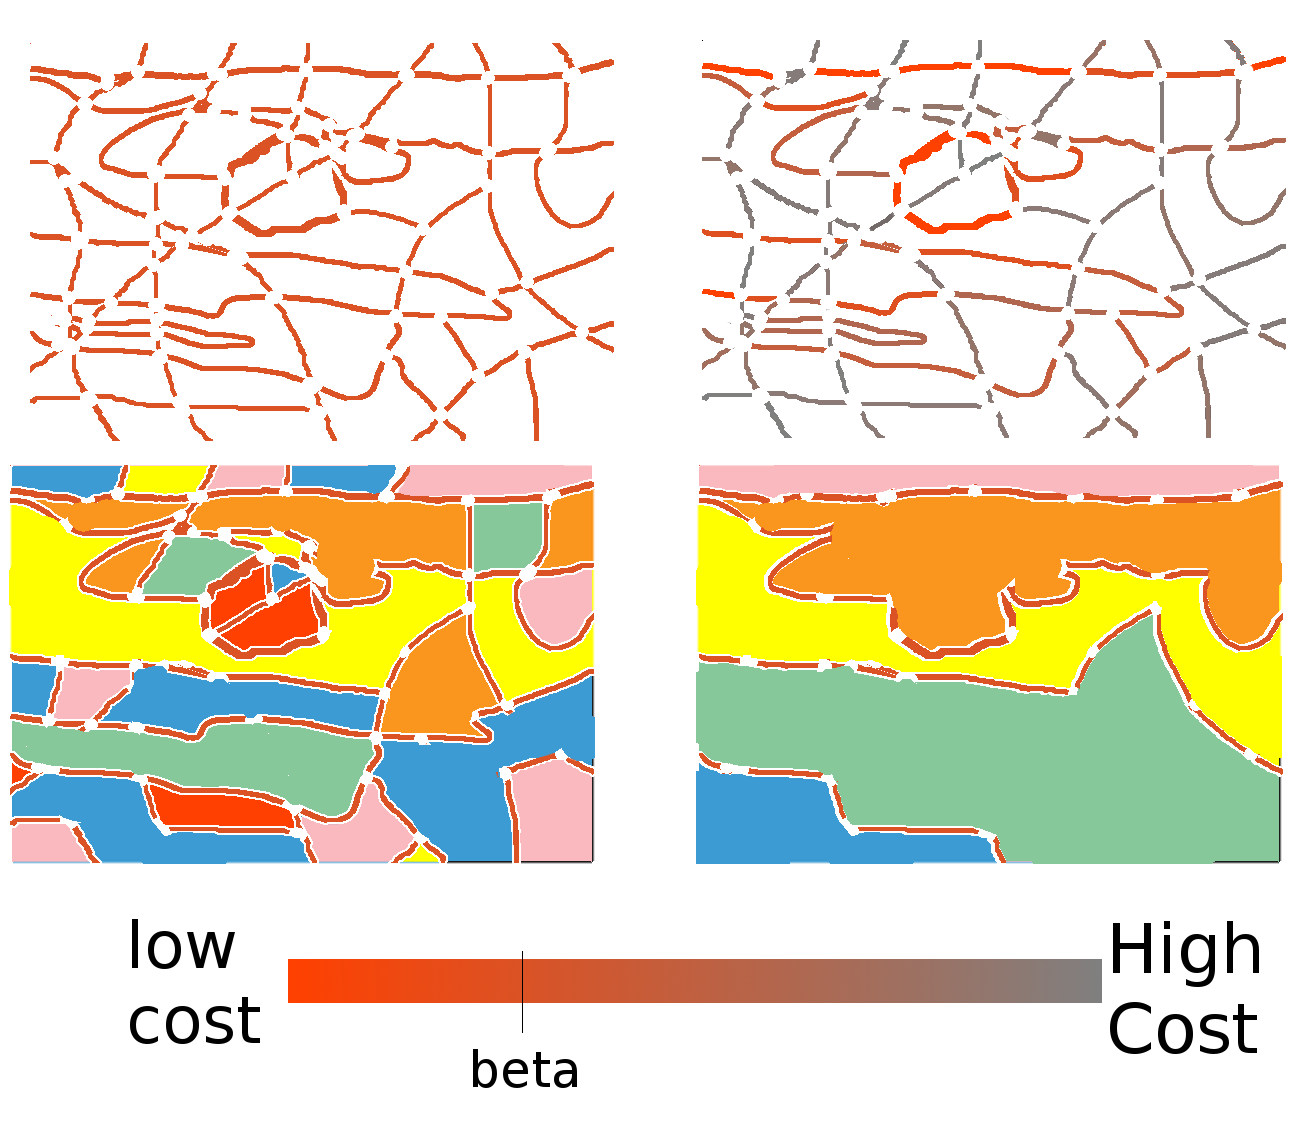
\includegraphics[width=\textwidth]{smooth} \caption[]%
        {{\small Pairwise term }}
        \label{fig:methodTerms:boundary}
    \end{subfigure}
    \caption {\small Methodology terms interpretation} 
    \label{fig:methodterms}
\end{figure}

In general, $\mathcal{S}$ can be any discrete set representing the image (i.e.\, pixels, overlapping or non overlapping windows, etc.). 
For this work $\mathcal{S}$ is chosen to be a super-pixels representation of the image.
Super-pixels can be seen as the output of an over-segmentation process or as a set of pixel collections that are contiguous and coherent with respect to a given metric. Either way, super-pixels are no overlapped irregular groups of similar connected pixels~\cite{achanta2012slic}.
\Cref{fig:methodTerms:problem} illustrates one such representation $\mathcal{S}$, applied to a \ac{bus} image example. The super-pixels are coloured according to the image's \ac{gt}.
For the rest of this work, $\mathcal{S}$ is considered to be the super-pixels resulting from an over-segmentation of the image using Quick-shift~\cite{massich2013phd}.

Bear in mind that given an unseen \ac{bus} image, the ultimate goal is to represent the image as a set of super-pixels and infer the appropriated labelling for each of them.
This goal requires to define: a data term, a pairwise term, and a proper minimization methodology.

\subsection{The data term} \label{sec:method:dataTerm}

Given a label configuration $\omega \in \mathcal{W}$, the data term penalizes the labelling of a particular image element or site ($\omega_s = l$) based on the data associated to $s$.
In this manner, $D_s(\omega_s=l_\cmark) << D_s(\omega_s=l_\xmark)$.
\Cref{fig:methodTerms:data} illustrates the data cost associated to some arbitrary labelling configurations to clarify the desired effect (or behaviour) of this data term (\cref{fig:methodTerms:problem} shows the \ac{gt} of each site $s$).
Notice that the labelling configurations $\omega$ used in \cref{fig:methodTerms:data} have the particularity that all sites share the same label, $\omega \in \{ \omega_s=l,~\forall s\in\mathcal{S}\}$.

Designing an obscure heuristic to comply with the desired behaviour of $D(\cdot)$ out of the box, is rather a complicated task.
Therefore, an easier and cleaner approach is to take advantage of \ac{ml} techniques to design this data cost in a systematic manner based on a training stage. 
The idea is to generate a data model for each label (or class) in $\mathcal{L}$ from training samples, and let $D(\cdot)$ be a distance or goodness measure reflecting the likelihood for $s$ to belong to class $l$.
\ac{ml} offers a systematic but flexible approach to customize $D(\cdot)$.
Different features to represent the data, custom construction of the data models by using different classifiers, training techniques or including arbitrary constraints; can be used to achieve the desired data term without changing the overall scheme. 

Despite details regarding the construction $D(\cdot)$ are out of the scope of this report, the rest of this \cref{sec:method:dataTerm} summarizes this process.
For further details the reader is referred to Massich et al.~\cite{massich2013phd}.
The usage of \ac{ml} as part of the proposed framework to determine $D(\cdot)$ is represented at the upper side of the diagram in~\cref{fig:method},
which can be divided into two blocks:
(a) the features to represent the samples,
and (b) the tools to encode $D(\cdot)$ based on the features and the training. 

\subsubsection{\ac{bus} features to build the data term} \label{sec:method:dterm:feat}
\Cref{fig:features} is a three-parts illustration to graphically summarize the visual cues that can be found in \ac{bus} images and their incorporation to the data term.
The structures of the breast and their rendering when using a hand-held 2D \ac{us} probe are shown in \cref{fig:features:breast}.
\Cref{fig:features:lexicon} illustrates the lexicon proposed by the \ac{acr}~\cite{biradsus}.
Whereas \cref{fig:features:relation} relates the visual cues to the following features:

\begin{description}
  \item[Appearance] 
    Based on the multi-labelled \ac{gt}, a \ac{mad} histogram model for every tissue label is build. The Appearance feature is computed as the \ac{qc} distance between histogram of $s$ and the models.
  \item[Atlas] 
    Based on the multi-labelled \ac{gt} an atlas is build to encode the label likelihood based on the location of $s$.
  \item[Brightness] 
    Takes an intensity descriptor of $s$ (\emph{i.e:} mean, median, mode) and compares it with some intensity markers of the set $\mathcal{S}$ such as the minimum intensity value, the maximum, its mean, etc.
  \item[\ac{sift}-\ac{bof}]
    $s$ is represented as the occurrences of a \ac{sift} dictionary of 36 words~\cite{massich2014sift}.
\end{description}

In order to incorporate multi-resolution, each super-pixel is group with its adjacent super-pixels such that $s' = \{s \cup \mathcal{N}_{s}\}$, the features are recalculated using $s'$ and concatenated to the original feature descriptor of $s$.
This operation can be repeated several times.

\begin{figure}
    \centering
    \begin{subfigure}[b]{0.34\textwidth}
        \centering
        \begin{tikzpicture}
          \node[inner sep=0, draw] (breast) {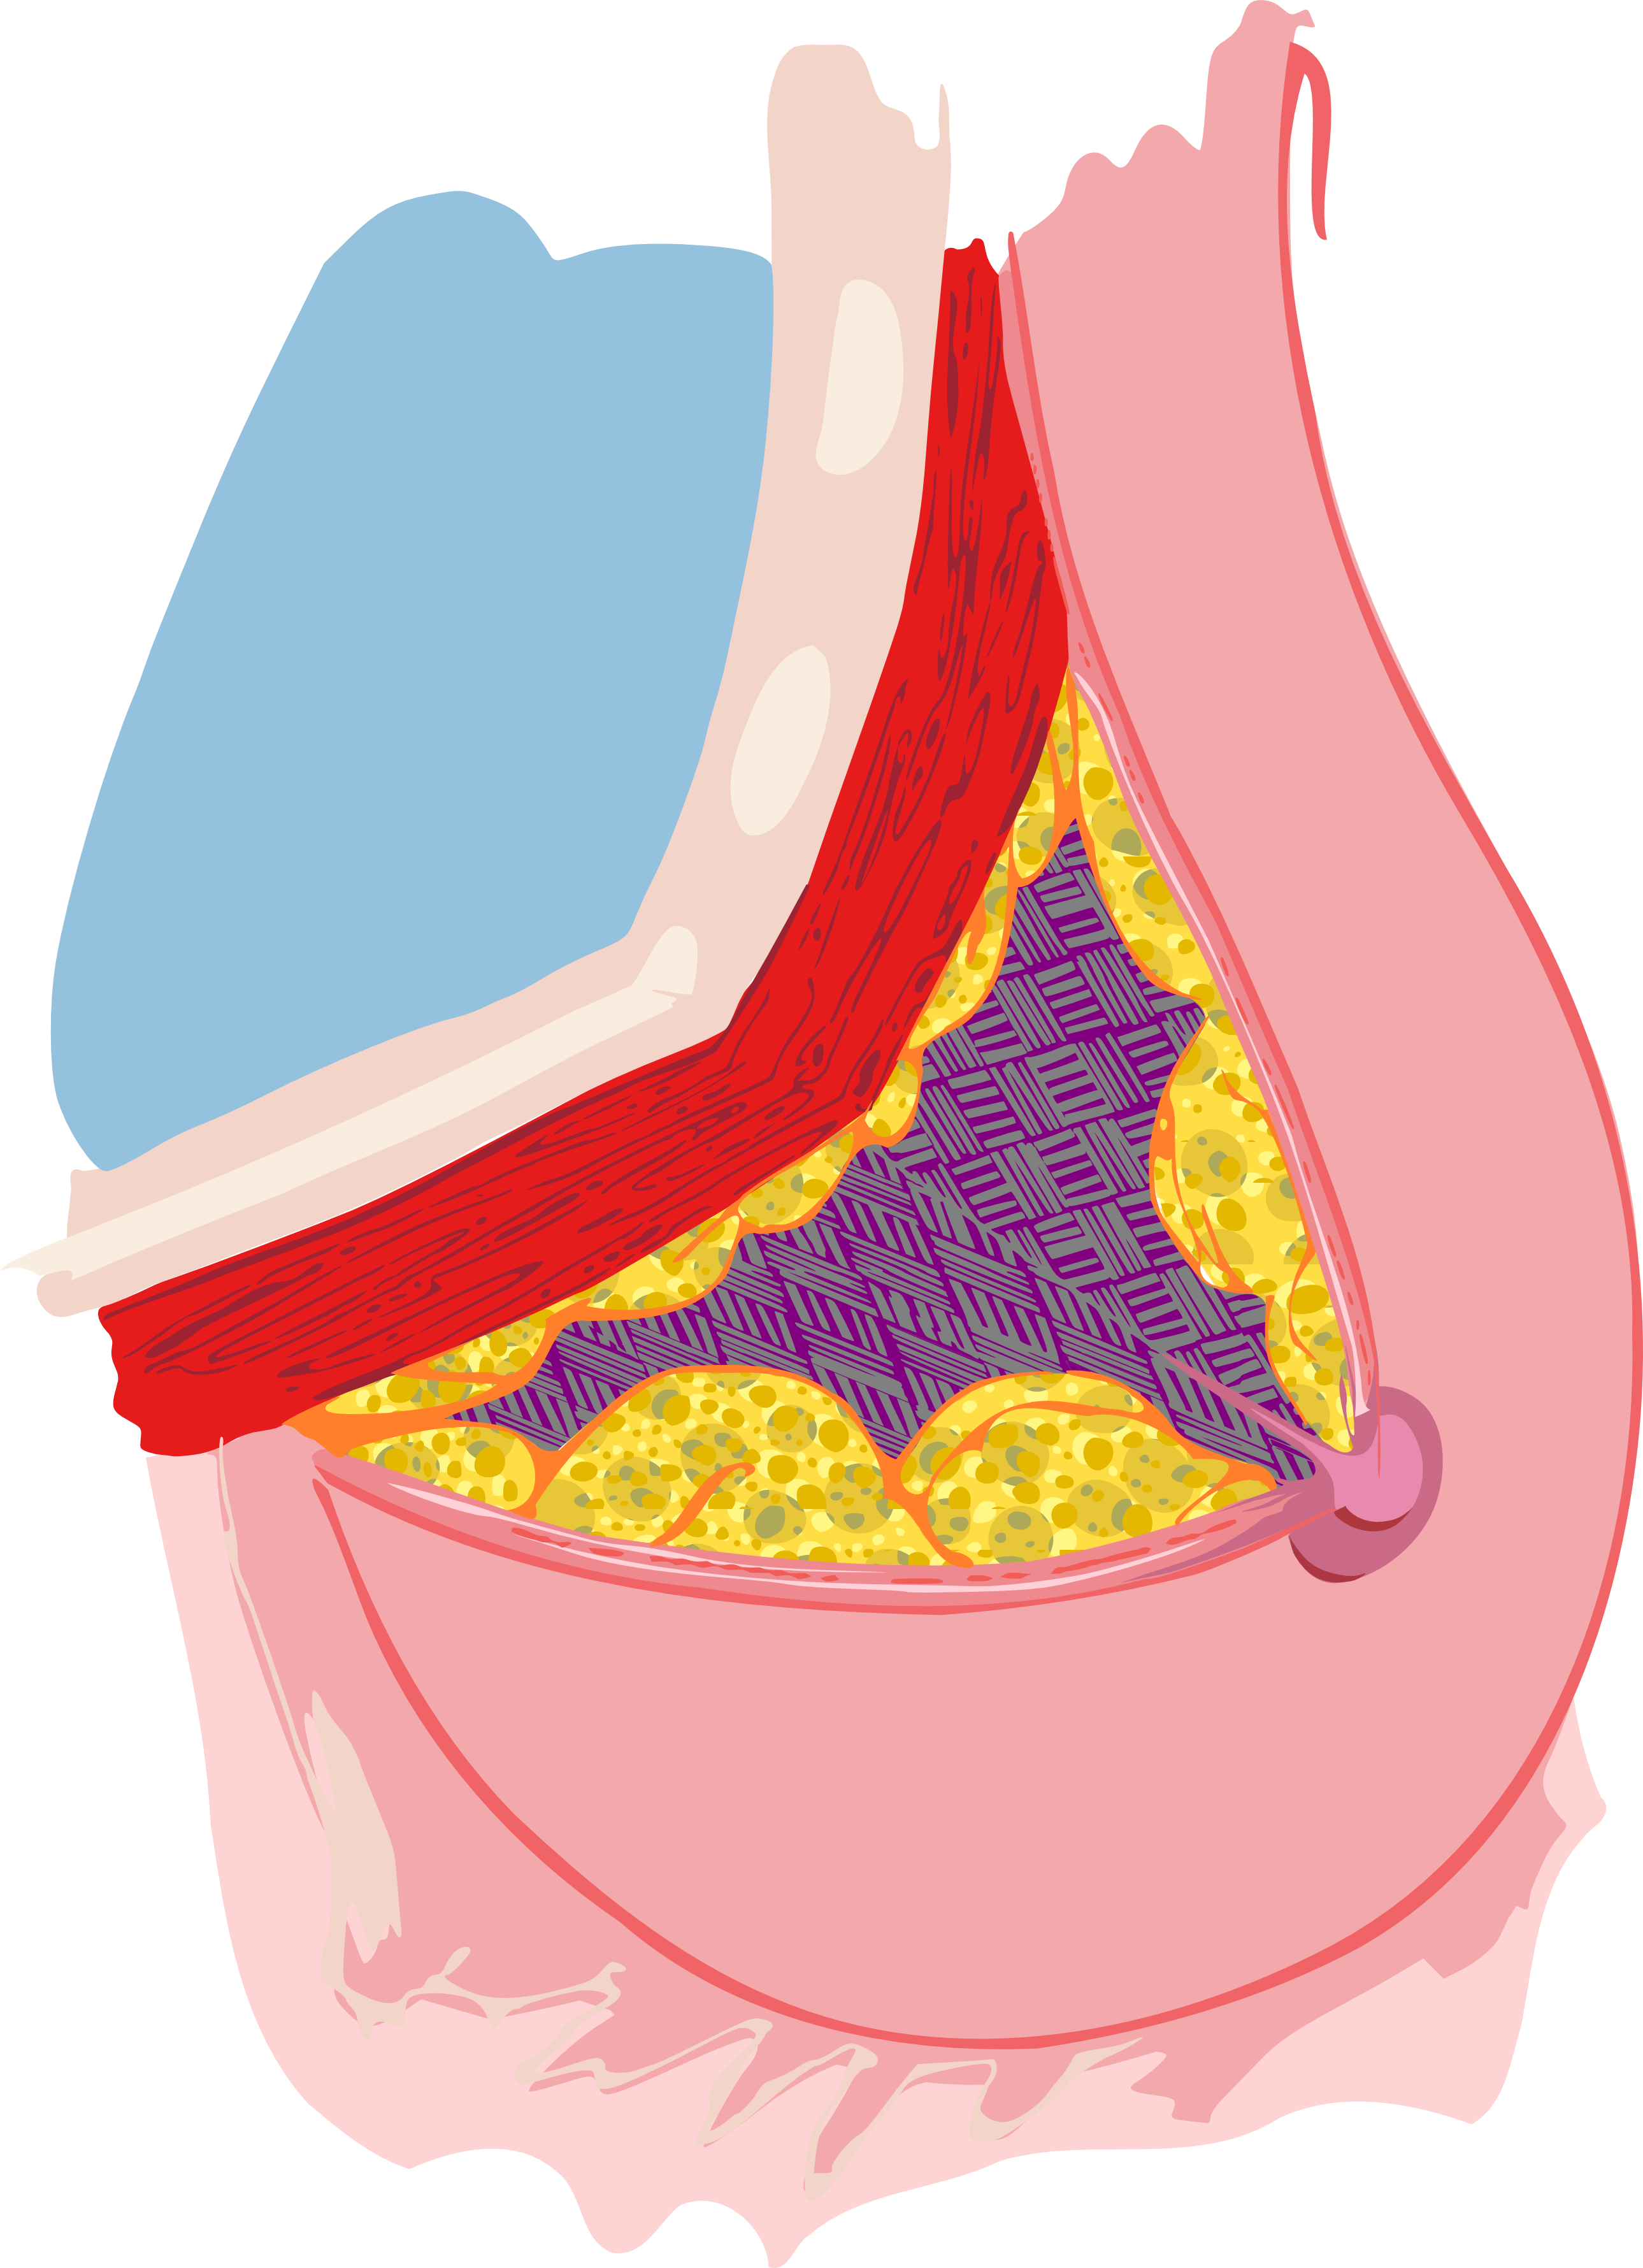
\includegraphics[width=0.5\textwidth]{breast}};
          \node[inner sep=0, draw, below= of breast] (slice) {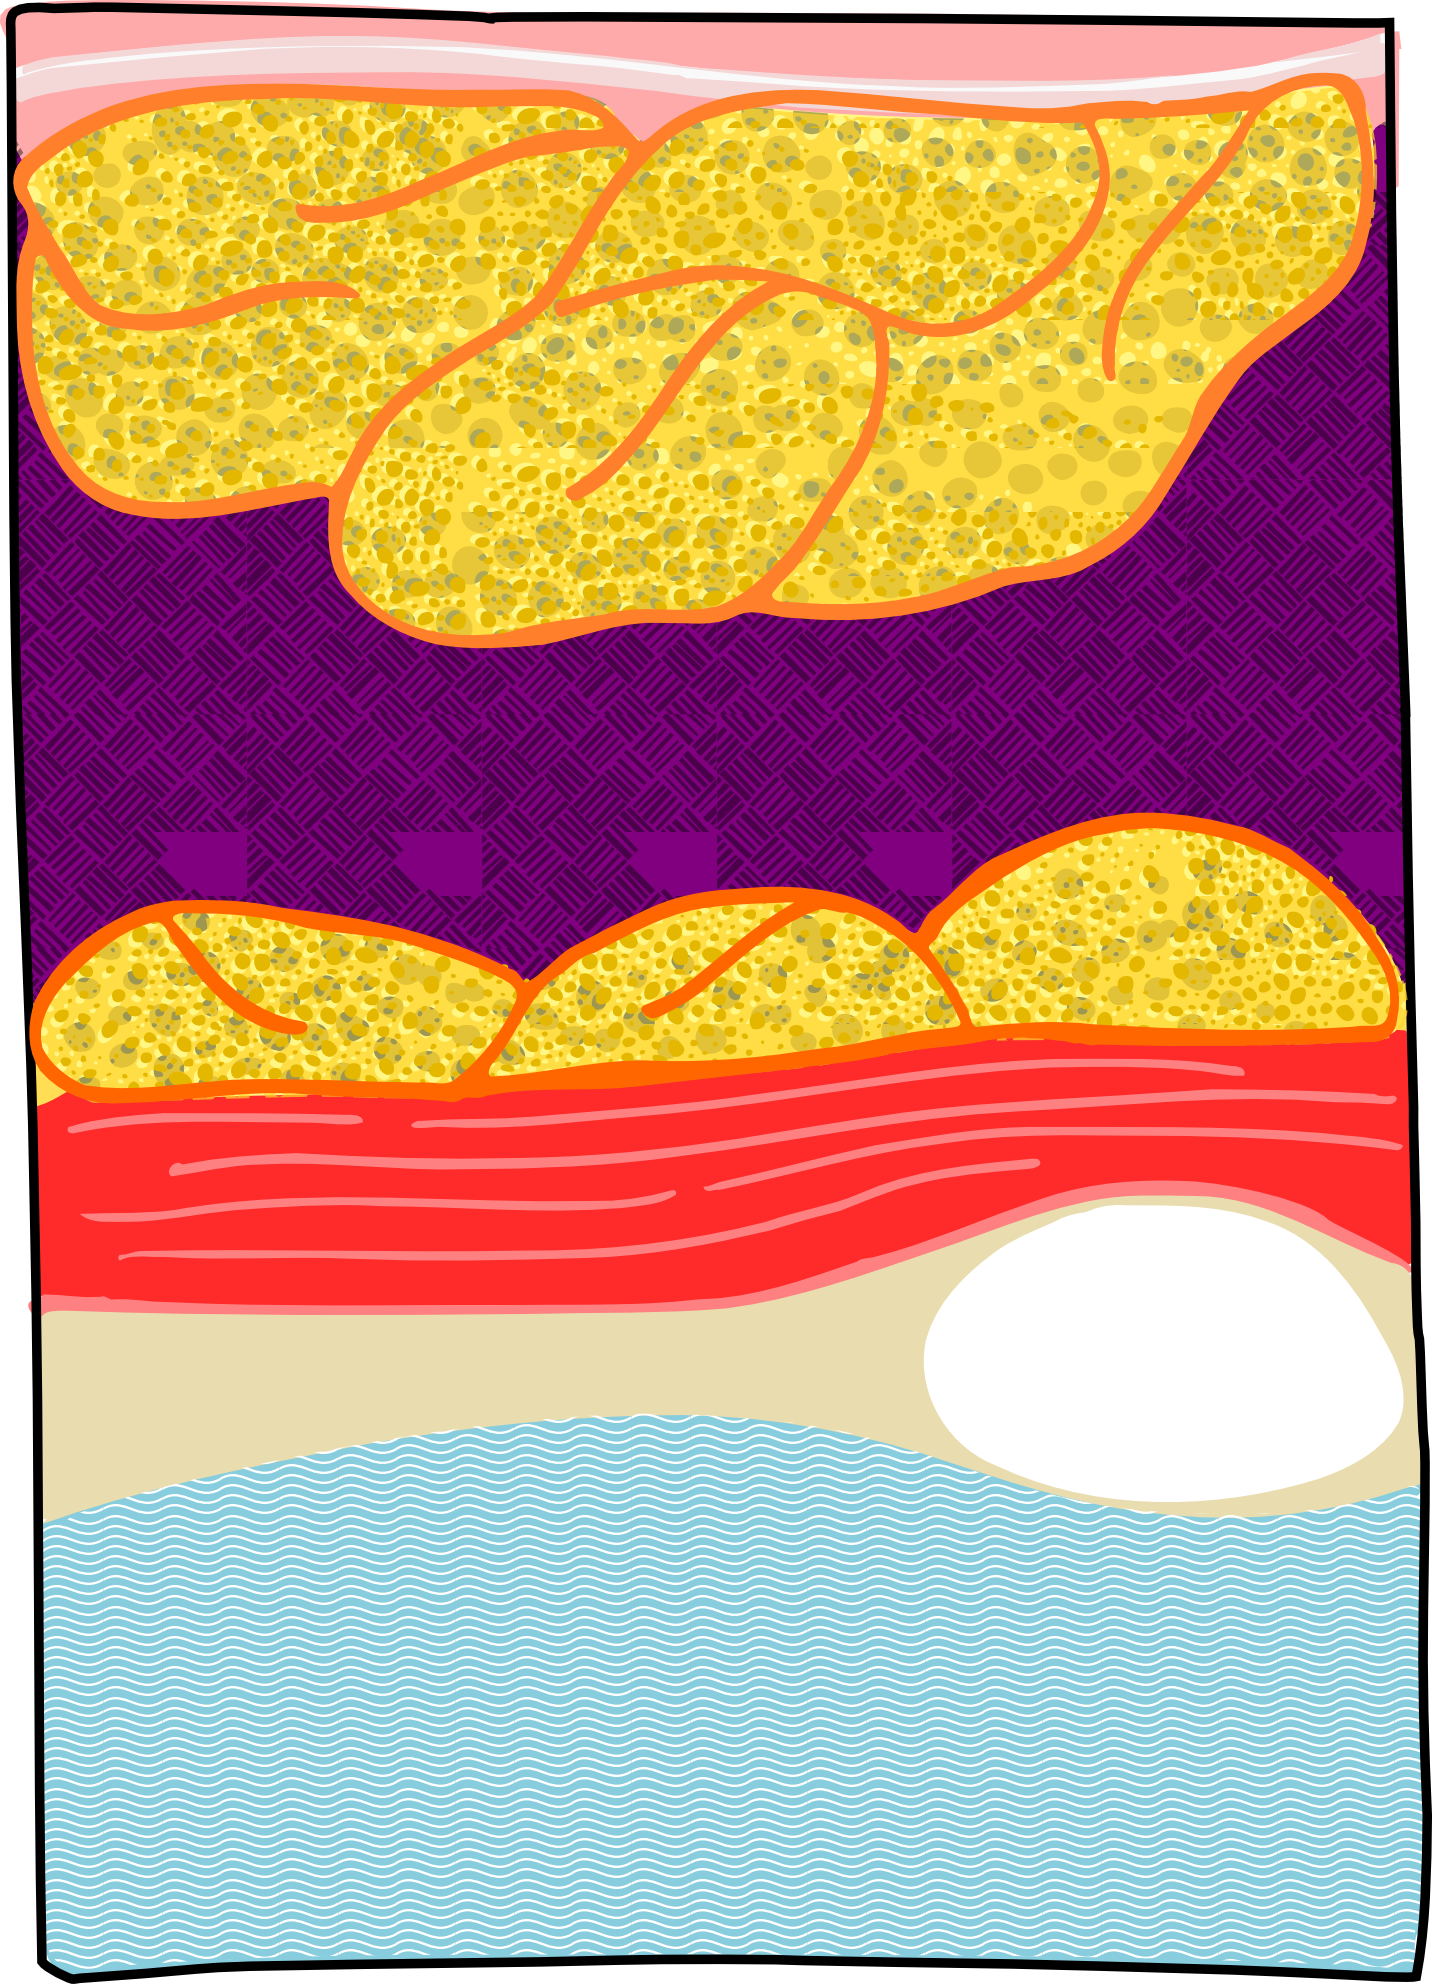
\includegraphics[width=0.5\textwidth]{slice}};
        \end{tikzpicture}
        \caption{{\small Breast structure}}    
        \label{fig:features:breast}
    \end{subfigure}
    \hfill
    \begin{subfigure}[b]{0.4\textwidth}   
        \centering 
        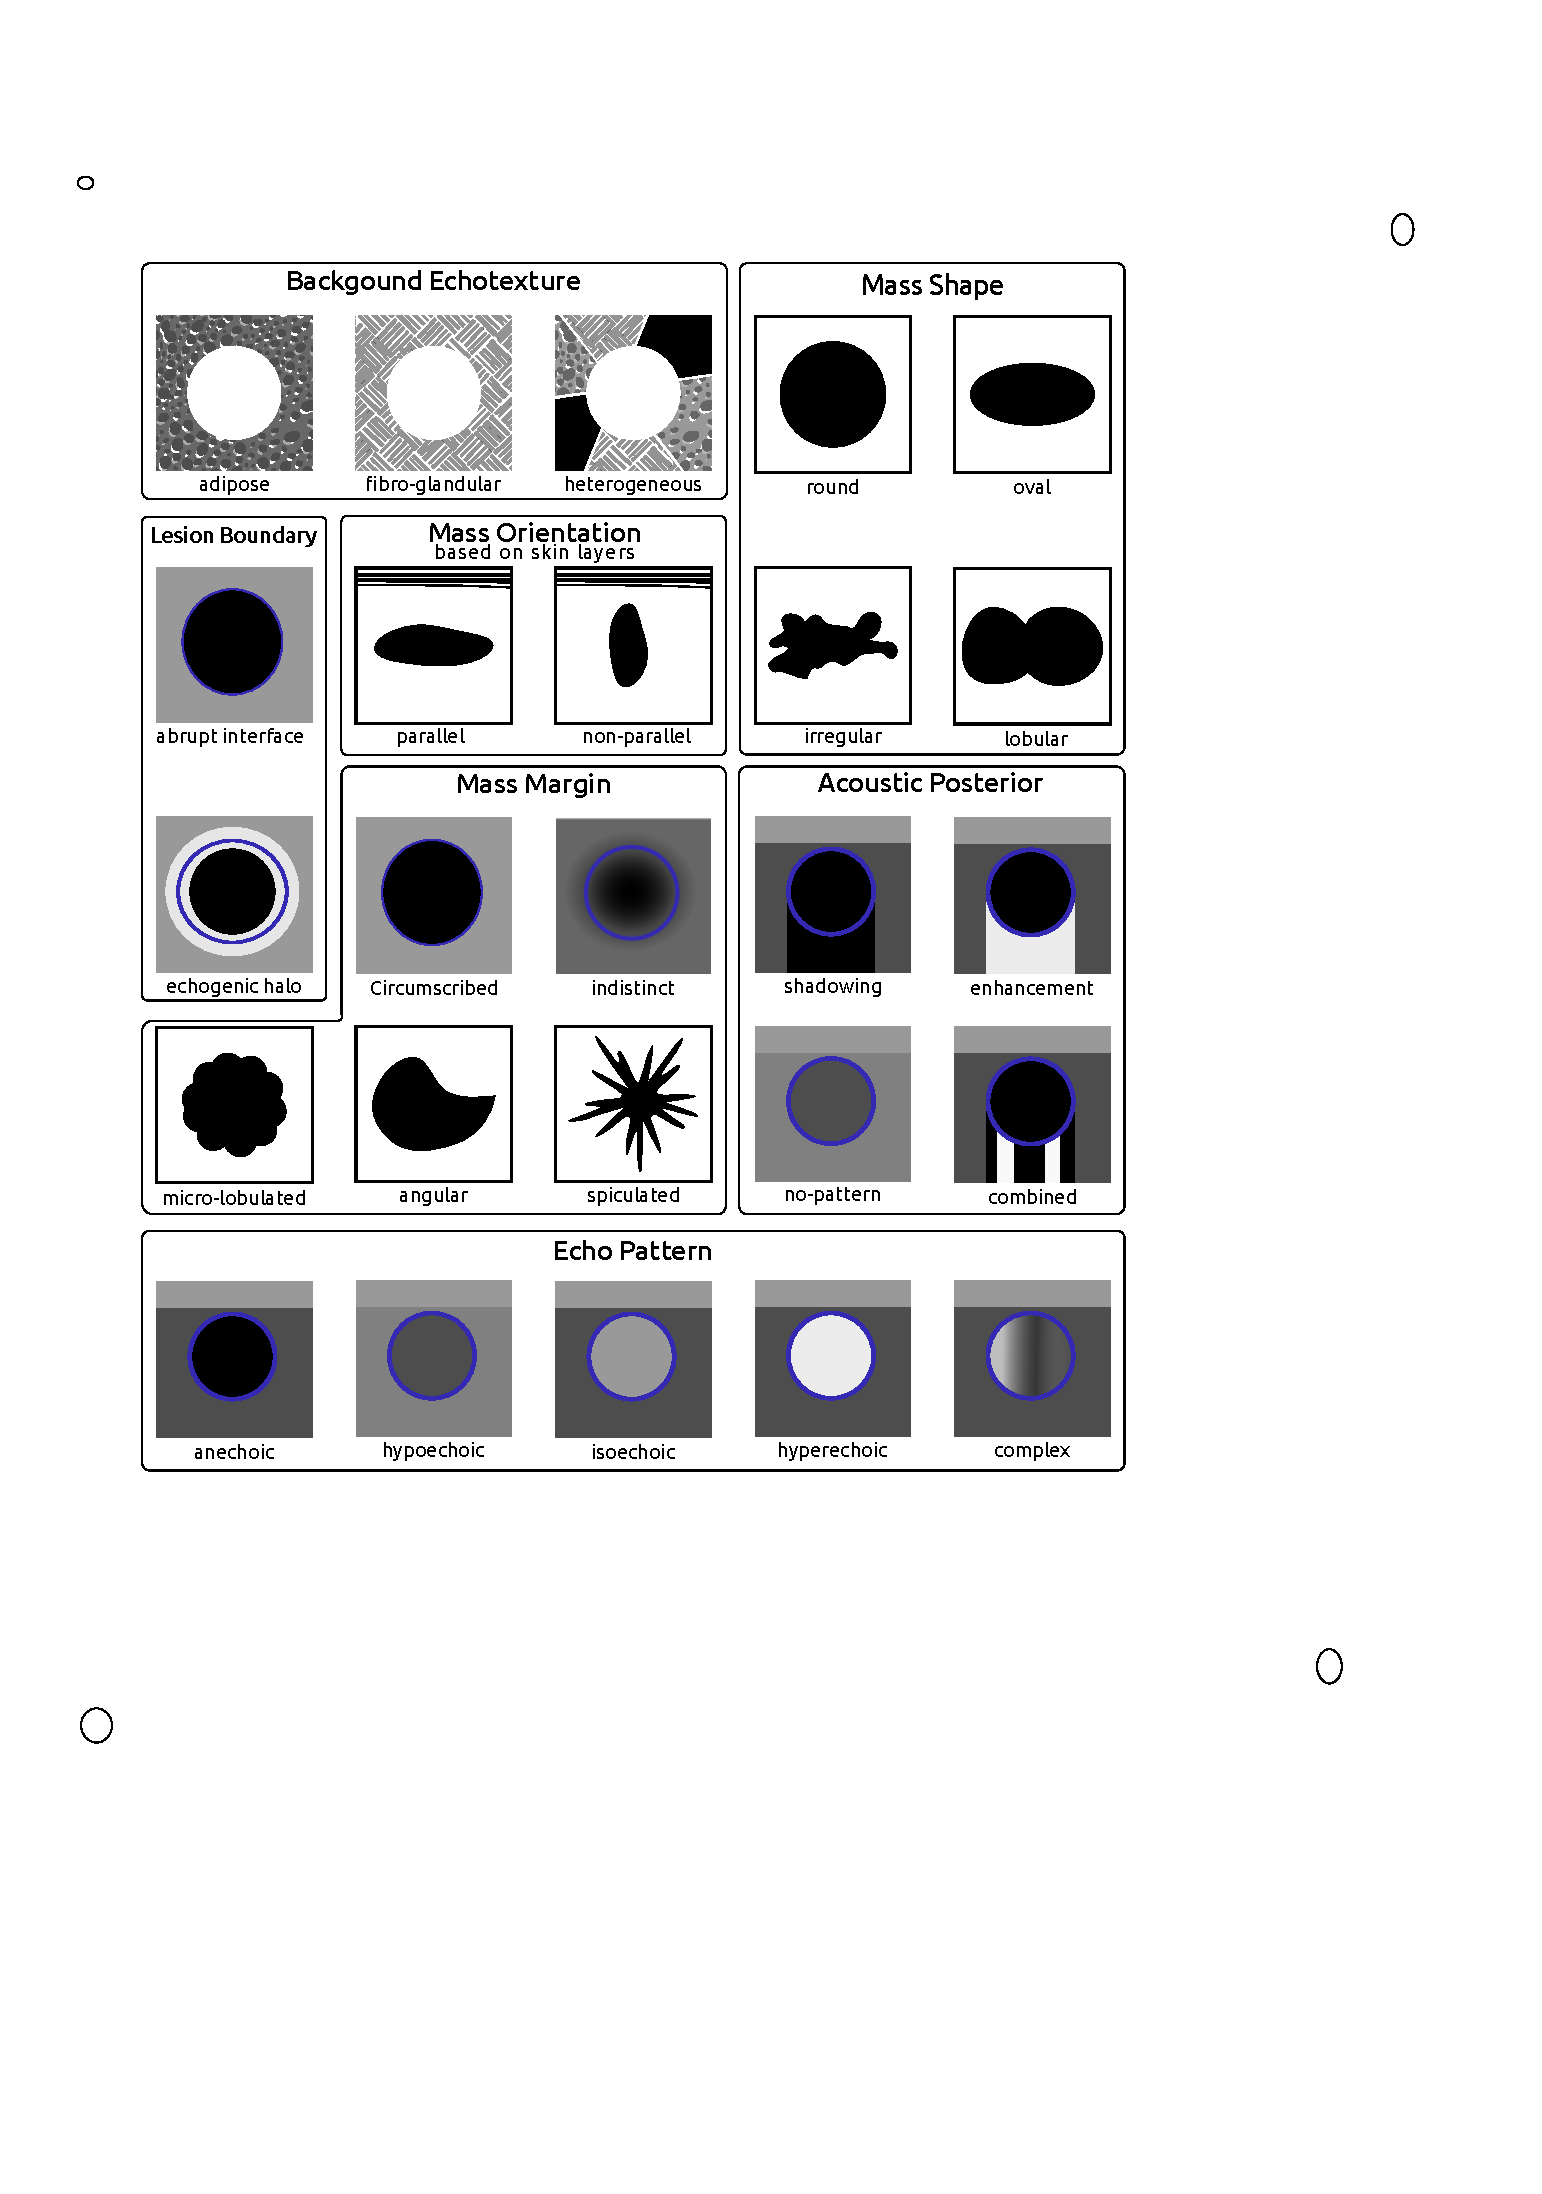
\includegraphics[trim = 65 345 200 124, clip,width=\textwidth]{birads}
        \caption[]%
        {Breast lesion characteristics in \ac{us} screening influencing clinical management~\cite{raza2010us}}    
        \label{fig:features:lexicon}
    \end{subfigure}
    \hfill
    \begin{subfigure}[b]{0.2\textwidth}
      \newcommand{\insertVisualCue}[2]{
        \tikz{\node[label=above:#2]{\includegraphics[width=0.5\textwidth]{#1}};}
      }
      \centering
      \begin{small}
        \insertVisualCue{AppearanceCues}{Appearance}
        \vfill
        \insertVisualCue{AtlasCues}{{Atlas, Brightness}}
        \vfill
        \insertVisualCue{siftCues}{SIFT-BoF}
      \end{small}
      \caption{Visual cues encoded in the features}
      \label{fig:features:relation}
    \end{subfigure}
    \hfill
    \caption {{\small Visual reference of breast structures and visual cues used for standard \ac{bus} image assessment and diagnosis.}} 
    \label{fig:features}
\end{figure}

Notice that not all the visual cues compiled by the lexicon are suitable to build the data term.
Mass shape, orientation and margin cues do not characterize an individual super-pixel but a group of contiguous super-pixels sharing the same label.
Characterising super-pixels in those terms imply that super-pixels should be image elements of the same order as the lesions. 
This is not the case, since the bottom-line is to aggregate small regions to form the segmentation.
The lesion boundary cue falls at the other extreme.
To encode this visual cue as data term feature implies to use smaller super-pixels in order to be fully contained within the halo, limiting the discriminatory power of other features that need larger regions to build higher-level descriptors.
%These cues are more suitable for \ac{cade} stages. 

In this manner the B.Echo-texture, is mainly encoded by the SIFT-BoF but also through the Appearance feature since elements would have the same model.
Acoustic Posterior is mainly captured by the Brightness feature, but the Atlas also brings crucial information to compensate for intensity inhomogeneities caused by signal attenuation present in the most posterior parts of the image.
The Echo Pattern cue, encodes the echoginity of a region with respect to the adipose tissue. This can be found at the anterior part of the image with its echoginity is close to the middle of the spectrum. Appearance, Brightness and the Atlas account for such information.

\subsubsection{The data term construction}
For the work here reported, a \ac{svm} classifier is used to determine the data model during the training stage.
During the testing stage, $D_s(\omega_s=l)$ corresponds to the distance between the testing samples and the model associated to $l$ as the \ac{svm} classification reward. 

\subsection{The pairwise (or smoothing) term} \label{sec:method:mrfTerm}
 
The pairwise term represents the cost associated to $\omega_s$ taking into account the labels of its neighbour sites, $\omega_r$, $r \in \mathcal{N}_{s}$. 
This term models a \ac{mrf} or a \ac{crf}.
The typical form of this term, given in \cref{eq:smoothing}, is called homogenization which acts as a regularization factor favouring configurations that have a coherent labelling.

\begin{equation}
V_{s,r}(\omega_s,\omega_r) = 
\begin{cases}
    \beta, & \text{if } \omega_s \ne \omega_r\\
    0,              & \text{otherwise}
\end{cases}
\label{eq:smoothing}
\end{equation}

\Cref{fig:methodTerms:boundary} offers a visual interpretation of this cost.
The more fragmented is the segmentation $\omega$, the higher the overall pairwise term; since every boundary brings a penalization $\beta$ to the total cost $U(\omega)$.
In this manner the regularization term can be seen as a post-processing or denoising stage since that some sites will flip their labelling if the cost of fragmenting the regions is larger than the cost of adopting their neighbour's label. 

More sophisticated smoothing terms, where boundaries have different penalization based on site relations in $\mathcal{S}$ and image information as illustrated in \cref{fig:methodTerms:boundary}, are also naturally handled by the proposed framework~\cite{massich2013phd}.

% Review %contribute have different or variable costs (see \cref{fig:methodTerms:boundary}) are also possible by taking into account not only relations in $\mathcal{S}$ of but also image information (see \cref{fig:method}). 
%Further details can be found in \cref{sec:smoothing}.

\subsection{Searching the best labelling configuration} \label{sec:method:min}
Once defined $U(\omega)$ so that the cost for a particular labelling configuration $\omega$ can be computed, the problem of finding $\hat{\omega}$ corresponding to the global minimum of the space $\mathcal{W}$ of all possible labelling configurations needs to be faced. 

This problem falls into the category of \textbf{NP-hard} problems. 
% Good % The dimension of the solution space can be expressed as $||\mathcal{W}|| = ||\mathcal{L}||^{||\mathcal{S}||}$. 
% Good % This means that in order to perform an exhaustive search for a toy example of $20$ sites and two possible labels, the cost function needs to be calculated way more than a million times. 
Moreover, due to limitations in building $U(\cdot)$ such as noise, training policies, etc. there are no guarantees that the global minimum $\hat{\omega}$ corresponds to the true labelling.

Nevertheless, there is a large body of literature proposing methodologies to find suboptimal solutions to the problem trading-off between time of convergence and accuracy of the solution reached.
Szeliski et al.~\cite{szeliski2008comparative} conducted an exhaustive review in terms of solution quality and runtime of the most common energy minimization algorithms used in \ac{cv}, such as \ac{icm}, \ac{sa} or \ac{gc}.

The minimization strategy used for this work is \ac{gc}. 
This technique was initially introduced to solve \ac{cv} applications by Boykov et al.~\cite{boykov2001fast}.
Soon after its introduction, it becomes the minimization technique of choice for \ac{cv} problems.
Since, when \ac{gc} is applicable, it allows to rapidly find a strong local minima guaranteeing that no other minimum with lower energies can be found~\cite{delong2012fast}. 
\ac{gc} is applicable if, and only if, the pairwise term favours coherent labelling configurations and penalizes labelling configurations where neighbours labels differs; 
such is our case, given in \cref{eq:smoothing}.

% Good % \subsection{Similitude with other optimization techniques}
% Good % \todo{needs reworking}
% Good % It is worth to mention here, that this pairwise term links this segmentation strategy to the family of segmentation methodologies based on optimization using \ac{acm}, such as levelsets.
% Good % On its basic form, the family of \ac{acm} segmentation defines some forces to be applied to an initial contour and this contour evolves by minimizing its length while constrained by the forces properly designed for the task in hand.

%%% Local Variables: 
%%% mode: latex
%%% TeX-master: "../../master.tex"
